% When Language Models Quote Uncertainty (working title; R5-1, D133). Project name: Quoting Volatility.
% Build:  uv run python scripts/paper/build.py && cd paper && tectonic main.tex      (or: latexmk -pdf main.tex)
% Every number in the text is a generated value (\pv{...}, paper/generated/macros.tex) or sits in a generated table
% or figure (paper/generated/); paper/generated/SOURCES.md lists the committed files each one was built from.
\documentclass[11pt]{article}
\usepackage{iftex}
\ifPDFTeX
  \usepackage[T1]{fontenc}
  \usepackage[utf8]{inputenc}
\fi
\usepackage{lmodern}
\usepackage[margin=1in]{geometry}
\usepackage{microtype}
\usepackage{amsmath,amssymb}
\usepackage{booktabs}
\usepackage{longtable}
\usepackage{array}
\newcolumntype{L}[1]{>{\raggedright\arraybackslash}p{#1}}
\usepackage{graphicx}
\usepackage{xcolor}
\usepackage[section]{placeins}
\usepackage[retain-explicit-plus=true, group-separator={,}, group-minimum-digits=4, group-digits=integer]{siunitx}
\usepackage[numbers,sort&compress]{natbib}
\usepackage{enumitem}
\usepackage[font=small,labelfont=bf]{caption}
\usepackage[hidelinks]{hyperref}

% Generated values: \pv{key} prints a value from paper/generated/macros.tex; an undefined key stops the build.
\makeatletter
\newcommand{\defpv}[2]{\expandafter\def\csname pv@#1\endcsname{#2}}
\newcommand{\pv}[1]{\@ifundefined{pv@#1}{\PackageError{paper}{Undefined generated value `#1'}{Rebuild
  paper/generated with scripts/paper/build.py.}}{\csname pv@#1\endcsname}}
\makeatother
% GENERATED by scripts/paper/macros.py; do not edit. Rebuild: uv run python scripts/paper/build.py
% artifact: macros
% sources (path @ git blob):
%   DECISIONS.md @ 4add2b31008a
%   FINDINGS.md @ d3660390b89c
%   configs/base_4bit.yaml @ 3d9d1725e751
%   configs/base_llama32_3b_4bit.yaml @ 584299a76a2e
%   configs/env_v2.yaml @ 547e903d8e18
%   configs/grpo_e1a.yaml @ e460668aa3e5
%   configs/grpo_e1d.yaml @ f13534dc12ad
%   configs/grpo_split_credit.yaml @ 3b36da32e485
%   configs/mc_a.yaml @ 45c25056e018
%   configs/mc_b.yaml @ 5d7b9a81130f
%   configs/pairs.yaml @ d305fb030896
%   configs/reward.yaml @ a5df0440dca2
%   configs/sft.yaml @ bb6d883bb58d
%   configs/sft_r4.yaml @ 065e0c38b078
%   configs/stage_a.yaml @ 00f62e8a0ad3
%   configs/stage_r4.yaml @ 8fa9146fcc1c
%   data/eval_sets/2.0.0+bdbb2279/confirmatory/a6_pairs_manifest.json @ a4667a2fef54
%   data/eval_sets/2.0.0+bdbb2279/confirmatory/a6b_pairs_manifest.json @ f42552284794
%   data/eval_sets/2.0.0+bdbb2279/confirmatory/a6c_pairs_manifest.json @ e413b9b471bf
%   data/eval_sets/2.0.0+bdbb2279/confirmatory/r5_6/a6b_pairs_manifest.json @ 33486465e0b3
%   data/eval_sets/2.0.0+bdbb2279/confirmatory/r5_6/a6c_pairs_manifest.json @ 3e36aa054364
%   data/jacobian_support/r4_1.json @ 68c4584bf672
%   physcal/env/formulas/dynamics.py @ 1df5803da9d5
%   physcal/env/formulas/energy.py @ 352ee72aefc0
%   physcal/env/formulas/kinematics.py @ 73721bf1f2b0
%   results/phase12_sft_data_r4/manifest.json @ f305c1b4036e
%   results/r5_diag/tail.json @ d92087ff65fd
%   results/sigma_star_gate_final/gate.json @ a7d0943a955d
%   results/stage_a/results.json @ e25937f751cb
%   results/stage_r4/dpos2/seed0/summary.json @ dcf5e628d3e5

\makeatletter
\defpv{eone.lr}{\num{5e-06}}% grpo_e1a.yaml grpo.learning_rate
\defpv{eone.lrd}{\num{5e-05}}% grpo_e1d.yaml grpo.learning_rate
\defpv{eone.steps}{\num{300}}% grpo_e1a.yaml grpo.max_steps
\defpv{eone.suffix}{\num{24}}% grpo_e1a.yaml grpo.max_completion_length
\defpv{frozen.aSix.problems}{\num{1020}}% confirmatory/a6_pairs_manifest.json n_problems
\defpv{frozen.aSixB.problems}{\num{1020}}% confirmatory/a6b_pairs_manifest.json n_problems
\defpv{frozen.aSixC.problems}{\num{1020}}% confirmatory/a6c_pairs_manifest.json n_problems
\defpv{gap.rss}{\num{0.00296}}% r5_diag/tail.json rss_to_star_gap
\defpv{gate.cov.one}{\SI{68.32}{\percent}}% gate.json primary_sigma_crps.levels.1.pooled.coverage
\defpv{gate.cov.two}{\SI{95.71}{\percent}}% gate.json primary_sigma_crps.levels.2.pooled.coverage
\defpv{gate.kupiec.one}{\num{0.92}}% gate.json primary_sigma_crps.levels.1.pooled.p
\defpv{gate.kupiec.two}{\num{0.20}}% gate.json primary_sigma_crps.levels.2.pooled.p
\defpv{gate.n}{\num{10005}}% gate.json n_noisy
\defpv{gate.ncells}{\num{15}}% gate.json config depths x levels
\defpv{gate.nominal.one}{\SI{68.27}{\percent}}% gate.json primary_sigma_crps.levels.1.pooled.nominal
\defpv{gate.nominal.two}{\SI{95.45}{\percent}}% gate.json primary_sigma_crps.levels.2.pooled.nominal
\defpv{gate.nzero}{\num{500}}% gate.json noise_zero.n
\defpv{gate.percell}{\num{667}}% gate.json config n_per_cell
\defpv{gate.pitp}{\num{0.98}}% gate.json pit.ks_p
\defpv{gen.distractors}{\num{0}--\num{2}}% env_v2 distractors
\defpv{gen.families}{kinematics, dynamics, energy}% pairs.yaml export.families
\defpv{gen.heldoutdepth}{\num{5}}% env_v2 splits.heldout_depths
\defpv{gen.kappa}{\num{5}}% env_v2 max_condition_number
\defpv{gen.levels}{\SI{1}{\percent}, \SI{2}{\percent}, \SI{5}{\percent}}% pairs.yaml export.levels (D54)
\defpv{gen.maxdepth}{\num{5}}% env_v2 splits.depths
\defpv{gen.maxlevel}{\SI{5}{\percent}}% pairs.yaml export.levels (D54)
\defpv{gen.mixedlevels}{\SI{0}{\percent}, \SI{1}{\percent}, \SI{2}{\percent}, \SI{5}{\percent}}% sft_r4.yaml mixed_levels (D113)
\defpv{gen.nfamilies}{\num{3}}% pairs.yaml export.families
\defpv{gen.nformulas.dynamics}{\num{15}}% physcal/env/formulas/dynamics.py FORMULAS
\defpv{gen.nformulas.energy}{\num{10}}% physcal/env/formulas/energy.py FORMULAS
\defpv{gen.nformulas.kinematics}{\num{12}}% physcal/env/formulas/kinematics.py FORMULAS
\defpv{gen.nmc}{\num{4000}}% env_v2 noise.n_mc
\defpv{gen.noisesigfigs}{\num{5}}% env_v2 noise.sig_figs
\defpv{gen.sigfigs}{\num{3}}% env_v2 display.sig_figs
\defpv{gen.version}{2.0.0}% env_v2 generator.version
\defpv{grpo.G}{\num{8}}% grpo_split_credit.yaml grpo.num_generations
\defpv{grpo.beta}{\num{0}}% grpo_split_credit.yaml grpo.beta
\defpv{grpo.ema}{\num{0.1}}% grpo_split_credit.yaml curriculum.alpha
\defpv{grpo.floor}{\num{0.02}}% grpo_split_credit.yaml curriculum.weight_floor
\defpv{grpo.lr}{\num{5e-06}}% grpo_split_credit.yaml grpo.learning_rate
\defpv{grpo.maxlen}{\num{512}}% grpo_split_credit.yaml grpo.max_completion_length
\defpv{grpo.prompts}{\num{4}}% grpo_split_credit.yaml grpo.prompts_per_step
\defpv{grpo.step}{\num{287}}% grpo_split_credit.yaml grpo.permanent_save_steps
\defpv{grpo.temp}{\num{1.0}}% grpo_split_credit.yaml grpo.temperature
\defpv{j.inv.exc}{\num{0.34}}% r5_6/a6b_pairs_manifest.json distances exceedance median
\defpv{j.inv.ntrain}{\num{3}}% r5_6/a6b_pairs_manifest.json distances n_training median
\defpv{j.inv.pairs}{\num{408}}% confirmatory/r5_6/a6b_pairs_manifest.json n_pairs
\defpv{j.inv.problems}{\num{816}}% confirmatory/r5_6/a6b_pairs_manifest.json n_problems
\defpv{j.margin}{\num{0.1}}% pairs.yaml j_jacobian.margin (D147 sec. 2)
\defpv{j.maxdepth}{\num{4}}% pairs.yaml j_allocation_export.depths
\defpv{j.scale.max}{\num{8}}% pairs.yaml j_invariance_construction.scale_factors
\defpv{j.scale.min}{\num{2}}% pairs.yaml j_invariance_construction.scale_factors
\defpv{j.sens.exc}{\num{0.38}}% r5_6/a6c_pairs_manifest.json distances exceedance median
\defpv{j.sens.ntrain}{\num{3}}% r5_6/a6c_pairs_manifest.json distances n_training median
\defpv{j.sens.pairs}{\num{408}}% confirmatory/r5_6/a6c_pairs_manifest.json n_pairs
\defpv{j.sens.problems}{\num{816}}% confirmatory/r5_6/a6c_pairs_manifest.json n_problems
\defpv{j.support.chains}{\num{1149}}% data/jacobian_support/r4_1.json chains
\defpv{j.worlds}{\num{96}}% pairs.yaml j_allocation_construction.candidate_worlds
\defpv{lora.alpha}{\num{16}}% stage_r4 lora.alpha
\defpv{lora.modules}{\num{7}}% stage_r4 lora.target_modules
\defpv{lora.r}{\num{16}}% stage_r4 lora.r
\defpv{mca.k}{\num{8}}% mc_a.yaml k
\defpv{mca.mad}{\num{1.4826}}% mc_a.yaml mad_scale
\defpv{mcb.exdepth}{\num{2}}% mc_b.yaml prompt.examples.cells depth
\defpv{mcb.nexamples}{\num{2}}% mc_b.yaml prompt.examples.cells
\defpv{mcb.tokens}{\num{640}}% mc_b.yaml generation.max_new_tokens
\defpv{model.base}{Qwen2.5-Math-1.5B-Instruct}% configs/base_4bit.yaml repo_id
\defpv{model.bits}{\num{4}}% configs/base_4bit.yaml repo_id (bnb-Nbit)
\defpv{model.llama}{Llama-3.2-3B-Instruct}% configs/base_llama32_3b_4bit.yaml repo_id
\defpv{pairs.aSix.ratio}{\num{2.0}}% pairs.yaml construction.min_ratio
\defpv{pairs.aSix.worlds}{\num{24}}% pairs.yaml construction.candidate_worlds
\defpv{pairs.aSixB.mc}{\num{1e-03}}% pairs.yaml invariance max_log_sigma_ratio
\defpv{pairs.aSixB.ratio}{\num{2.0}}% pairs.yaml invariance min_target_ratio
\defpv{pairs.aSixB.worlds}{\num{24}}% pairs.yaml invariance_construction.candidate_worlds
\defpv{pairs.aSixC.ratio}{\num{1.5}}% pairs.yaml allocation min_ratio
\defpv{pairs.aSixC.worlds}{\num{24}}% pairs.yaml allocation_construction.candidate_worlds
\defpv{pairs.cells}{\num{15}}% pairs.yaml export depths x levels
\defpv{pairs.percell}{\num{34}}% pairs.yaml export.pairs_per_cell
\defpv{record.dentries}{\num{150}}% DECISIONS.md: '### D<n>.' headers
\defpv{record.findings}{\num{39}}% FINDINGS.md: the highest '## #<n>.' header
\defpv{rfour.batch}{\num{8}}% stage_r4.yaml train batch x accumulation
\defpv{rfour.epochs}{\num{2}}% stage_r4.yaml train.epochs
\defpv{rfour.evalbatch}{\num{16}}% stage_r4.yaml eval.batch_size (D116)
\defpv{rfour.lr}{\num{1e-04}}% stage_r4.yaml train.learning_rate
\defpv{rfour.mixing}{\num{2067}}% phase12_sft_data_r4/manifest.json
\defpv{rfour.n}{\num{3000}}% phase12_sft_data_r4/manifest.json n_examples
\defpv{rfour.seeds}{\num{3}}% stage_r4.yaml confirmatory.seeds
\defpv{rfour.sfmt}{\num{3}}% sft_r4.yaml sensitivity_format (.Ng)
\defpv{rfour.steps}{\num{750}}% stage_r4/dpos2/seed0/summary.json steps_planned
\defpv{rfour.tokens}{\num{1280}}% stage_r4.yaml eval.long_max_new_tokens (D114)
\defpv{sa.draws}{\num{4000}}% stage_a.yaml mc.n_draws
\defpv{sa.halfwins}{\SI{44}{\percent}}% stage_a results.json resolution.0.5x_sigma_star realized share (1 - star better)
\defpv{sa.scale}{\num{2}}% stage_a.yaml alternatives.scales
\defpv{sa.varratio.max}{\num{23}}% stage_a results.json resolution.*.pooled.variance_ratio (max)
\defpv{sa.varratio.min}{\num{5}}% stage_a results.json resolution.*.pooled.variance_ratio (min)
\defpv{sft.lr}{\num{1e-04}}% sft.yaml train.learning_rate
\defpv{sft.minutes}{\num{30}}% sft.yaml train.wall_clock_minutes
\defpv{sft.n}{\num{3000}}% sft.yaml data.n_examples
\defpv{sft.sigmarel}{\SI{2}{\percent}}% sft.yaml data.sigma_rel
\defpv{split.ref}{\SI{1}{\percent}}% grpo_split_credit.yaml split_credit.sigma_ref_rel
\defpv{split.seeds}{\num{3}}% configs/grpo_split_credit*.yaml (one config per seed)
\defpv{stat.B}{\num{10000}}% stage_r4.yaml analysis.bootstrap
\defpv{stat.alpha}{\num{0.05}}% stage_r4.yaml analysis.alpha
\defpv{stat.cilevel}{\SI{90}{\percent}}% stage_r4.yaml analysis.criterion_ci_level
\defpv{stat.floor}{\num{1e-06}}% pairs.yaml analysis.sigma_floor_rel
\defpv{stat.margin}{\num{0.3}}% pairs.yaml invariance_analysis.equivalence_margin
\defpv{stat.practical}{\num{0.5}}% stage_r4.yaml analysis.practical_slope (C2)
\defpv{ver.binary}{\SI{1}{\percent}}% reward.yaml scoring.binary_tolerance
\defpv{ver.floor}{\num{-5}}% reward.yaml scoring.crps_clip
\defpv{ver.sigmafloor}{\num{1e-06}}% reward.yaml scoring.crps_log_sigma_floor
\defpv{ver.steptol}{\SI{2}{\percent}}% reward.yaml steps.tolerance
\defpv{ver.stepweight}{\num{0.2}}% reward.yaml weights.steps
\defpv{ver.tau}{\num{1e-03}}% pairs.yaml analysis.tau (D50/A1)
\defpv{ver.version}{1.1.0}% reward.yaml version
\makeatother


\newcommand{\sigstar}{\sigma^{\star}}
\newcommand{\crpslog}{\mathrm{crps}_{\log}}
\newcommand{\todo}[1]{\textcolor{gray}{\emph{[#1]}}}

\title{When Language Models Quote Uncertainty:\\Separating Reasoning Errors from Measurement Noise}
\author{Raghhav\thanks{Draft of \today. Author list and affiliations to be completed.}}
\date{}

\begin{document}
\maketitle

\begin{abstract}
\todo{Abstract to be written after the results sections.}
\end{abstract}

% Section: Introduction. NOT drafted yet (docs/paper_outline.md sec. 1; R5-1 framing).
\section{Introduction}
\label{sec:intro}
\todo{To be written. Outline: the question; why a benchmark with known $\sigstar$; the three findings, one per panel
of Figure~\ref{fig:headline}; contributions stated narrowly (docs/paper\_outline.md, section 1).}

% Section: Related work. NOT drafted yet (docs/paper_outline.md sec. 2). Every reference is verified before it is
% cited (R5-10, R4-9).
\section{Related work}
\label{sec:related}
\todo{To be written after the references in docs/paper\_outline.md, section 2, are verified (R5-10).}

% Section: Setup (drafted 2026-10-30). Every claim cites its source in a comment; every number is \pv{...}.
\section{Setup}
\label{sec:setup}

\subsection{A generator of physics problems with known uncertainty}
\label{sec:generator}

% Spec (CLAUDE.md, component 1); physcal/env/graph.py; D51 (generator 2.0.0); configs/env_v2.yaml.
The benchmark is a procedural generator of multi-step physics word problems (generator version \pv{gen.version}).
It has \pv{gen.nfamilies} formula families (\pv{gen.families}), each one physical scenario with named, dimensioned
quantities and a set of relations written in SymPy~\citep{meurer2017sympy}: \pv{gen.nformulas.kinematics},
\pv{gen.nformulas.dynamics} and \pv{gen.nformulas.energy} relations respectively.
% physcal/env/graph.py: Family.sample_world, chains, is_valid_chain.
A problem is a linear chain through its family's formula graph.
The generator samples a consistent world (basis quantities log-uniform within physical ranges, derived quantities
checked against plausibility bounds), picks a chain, shows the chain's inputs (the \emph{givens}) and asks for its
output (the \emph{target}).
The depth of a chain, from one step up to \pv{gen.maxdepth}, is its difficulty dial.
% graph.py docstring: "the target's minimal derivation depth ... must equal the chain length ... no given may be
% derivable from the other givens".
Depth is honest: the target's shortest derivation from the givens, over all relations of the family, has exactly
the chain's length, and no given can be derived from the others.
% env_v2 splits.heldout_depths; R5-8 (depth 5 is extrapolation in chain length, not to new physics).
Depth \pv{gen.heldoutdepth} is never used for training.
It tests extrapolation in chain length within the same families, not transfer to new physical laws.

% D10 (distractors), D11 (plausibility bounds), CLAUDE.md component 1 (units, phrasing), env_v2 display settings.
Each problem's text is randomized: phrasing templates, display units with SI prefixes and non-SI units, and
\pv{gen.distractors} distractor quantities that the answer does not depend on.
% env_v2 max_condition_number; physcal/env/graph.py condition_number.
Chains whose output amplifies relative errors in a given by more than a factor of \pv{gen.kappa}
(the largest $|\partial \ln(\text{output}) / \partial \ln(\text{given})|$) are rejected.
% physcal/env/graph.py evaluate_chain_with_units (pint dimension checks).
The ground truth is computed in SI units with dimension checks at every step, then converted to the requested unit.
Every problem is reproducible from its generator version and seed.

\subsection{Measurement noise and the true uncertainty $\sigstar$}
\label{sec:sigstar}

% D51 (noise mode: 5 s.f. so that rounding is negligible against the noise, FINDINGS #8; a problem without noise
% behaves as generator 1.1.0, 3 s.f., truth from the displayed values); D113 (mixed levels: every given at 5 s.f.,
% level-0 givens exact); D54 (levels capped at 5% after FINDINGS #9; a post-hoc design change); configs/pairs.yaml.
In the measurement-noise mode, each noisy given is shown as a measurement
$x_{\text{meas}} = x_{\text{true}}(1+e)$, $e \sim \mathcal{N}(0, s^2)$, with \pv{gen.noisesigfigs} significant
figures, so that rounding is negligible against the noise, and a stated relative uncertainty ``$\pm\, s$''; a value
shown without one is exact.
The truth is the noise-free chain evaluated on the unrounded true values.
A problem without noise shows \pv{gen.sigfigs} significant figures, and its truth is computed from the displayed
values.
The pair sets of Section~\ref{sec:pairs} use the levels \pv{gen.levels}, and the training data of
Section~\ref{sec:dpos} draws a level for each given independently from \pv{gen.mixedlevels}, where a level of zero
means an exact given.

% D50/A2 (sigma* definition), D51 (stored per problem; n_mc draws); JCGM 101 (propagation of distributions).
Because the generator knows the measurement model, it knows each problem's correct uncertainty.
Given the displayed values, the clean value of each noisy given is drawn as $x = x_{\text{meas}}/(1+e')$,
$e' \sim \mathcal{N}(0, s^2)$, with exact givens and constants held fixed; \pv{gen.nmc} such draws are pushed through
the chain, as in Monte Carlo propagation of distributions~\citep{jcgm101}.
The target $\sigstar$ is the scale of the Gaussian in log space, centred at $\ln f(x_{\text{meas}})$, that minimizes
the expected CRPS against these draws:
\begin{equation}
  \sigstar = \arg\min_{\sigma > 0}\; \mathbb{E}_{x}\!\left[\mathrm{CRPS}\!\left(\mathcal{N}(\ln f(x_{\text{meas}}),
  \sigma^2),\, \ln f(x)\right)\right],
  \label{eq:sigstar}
\end{equation}
where $f$ is the chain and $f(x_{\text{meas}})$ is what a correct solver computes from the displayed values.
% D50/A2: also stored, the SD of the log draws and the delta-method value (used to build the pair sets).
The standard deviation of the log draws and the first-order (delta-method) value are stored as well.

% D50/A3 (gate), D57 (miss-count rule; FINAL run), FINDINGS #12 (passed), #9 and #11 (the two failed runs);
% results/sigma_star_gate_final/gate.json.
Before any model was evaluated on noisy problems, the generator had to pass a self-consistency gate: intervals
$\ln f(x_{\text{meas}}) \pm k\sigstar$ must cover the clean truth at their nominal rates.
On the final run, with \pv{gate.n} noisy problems in \pv{gate.ncells} depth-by-level cells of \pv{gate.percell}
each, pooled coverage was \pv{gate.cov.one} at $k=1$ (nominal \pv{gate.nominal.one}, Kupiec~\citep{kupiec1995}
$p = \pv{gate.kupiec.one}$) and \pv{gate.cov.two} at $k=2$ (nominal \pv{gate.nominal.two},
$p = \pv{gate.kupiec.two}$).
No cell was rejected after Holm correction, and the probability integral transform of the truth was uniform
(Kolmogorov--Smirnov $p = \pv{gate.pitp}$).
The \pv{gate.nzero} noise-free control problems were exact.
% FINDINGS #9 (failed on one cell at 10% noise) -> D54 (cap at 5%, after the result); FINDINGS #11 (failed only on
% the cell-share rule, which demanded zero misses) -> D57 (miss-count test, before the final run).
The gate failed twice before this run.
The first run failed on one cell at the highest noise level, after which the noise levels were capped; that cap was
chosen after seeing the result.
The second failed only on a rule that, as written, tolerated no cell outside its interval; it was replaced by a
miss-count test before the final run.
Both changes are listed in Table~\ref{tab:deviations}.

\subsection{Output format and verifier}
\label{sec:verifier}

% CLAUDE.md component 3 (format); D16, D17 (parser); D83 (the <confidence> channel, verifier 1.2.0).
A completion may reason freely, then reports the requested intermediate values in a \texttt{<steps>} block and the
answer as \texttt{<answer>}$\mu \pm \sigma$ \textit{unit}\texttt{</answer>}.
% D13 (failures score the rule's floor); CLAUDE.md component 4 (units gate).
A completion that does not parse, or whose unit has the wrong dimension, scores the rule's floor
(\pv{ver.floor}); an answer in another unit of the right dimension is converted.

% D15 (the spec's relative CRPS is only approximately proper), D29 (crps_log is the default), D38 (its sigma floor);
% configs/reward.yaml; Gneiting & Raftery (2007); closed form of the Gaussian CRPS: Gneiting et al. (2005).
The scoring rule, $\crpslog$, scores the log of the truth $y$ against $\mathcal{N}(\ln\mu, (\sigma/\mu)^2)$:
\begin{equation}
  \crpslog(\mu,\sigma; y) = -\,s\left[z\left(2\Phi(z)-1\right) + 2\varphi(z) - \tfrac{1}{\sqrt{\pi}}\right],\qquad
  z = \frac{\ln y - \ln \mu}{s},\quad s = \max\!\left(\sigma/\mu,\ \epsilon\right),
  \label{eq:crpslog}
\end{equation}
the Gaussian CRPS in closed form~\citep{gneiting2005emos}, clipped below at the floor.
It is strictly proper for log-normal beliefs~\citep{gneiting2007strictly} and scale-free.
% D15: dividing by the truth reweights outcomes by 1/|y|; the optimal mu shifts and the optimal sigma inflates.
The relative CRPS of the original specification divides by the truth, which reweights outcomes and makes it only
approximately proper; it remains an ablation option.
% D37, D38: a floor of 0.1% made the reward flat in sigma for an overconfident policy; verifier 1.1.0 floors at 1e-6.
The floor $\epsilon$ is \pv{ver.sigmafloor} (verifier \pv{ver.version}): an earlier, larger floor made the reward
flat in $\sigma$ exactly where an overconfident policy needed a gradient.
% configs/reward.yaml weights and steps; D14 (step credit can never outweigh the final answer).
During reinforcement learning the reward adds \pv{ver.stepweight} times the share of requested intermediates within
\pv{ver.steptol} of their values; this weight is checked to be too small to ever outweigh the final score.
An answer is \emph{accurate} if it is within \pv{ver.binary} of the truth.

% D50/A1 (computation-correct subset); configs/pairs.yaml analysis.tau.
On noisy problems, an answer is \emph{computation-correct} if $|\ln\mu - \ln f(x_{\text{meas}})| \leq
\pv{ver.tau}$, that is, if it is what a correct solver computes from the displayed values.
Comparisons of a stated $\sigma$ with $\sigstar$ that require a correct answer use this subset.

\subsection{The oracle-centred expected score}
\label{sec:expected}

% FINDINGS #24 (stage A), D100; results/stage_a/results.json; results/r5_diag/tail.json (the gap).
A single realized truth says little about whether a stated $\sigma$ is right: a $\sigma$ that is \pv{sa.scale}
times too small scores better than $\sigstar$ against the realized truth on \pv{sa.halfwins} of problems.
Because the generator knows the predictive distribution, we also score a stated relative $\sigma$ by its
\emph{expected} $\crpslog$ over \pv{sa.draws} fresh predictive draws, centred at $f(x_{\text{meas}})$.
Per-problem differences between sources then have \pv{sa.varratio.min}--\pv{sa.varratio.max} times less variance than
the realized ones.
Expected-score differences are reported with their intervals and, where useful, as a share of the gap between the
noise heuristic RSS (Section~\ref{sec:comparators}) and $\sigstar$, which is \pv{gap.rss} on the frozen
confirmatory set.

\subsection{Counterfactual pair sets}
\label{sec:pairs}

% D50/A6, D58 (A6), D59 (A6b), D95 (A6c), D113 (the frozen confirmatory set), D147 (the J set);
% configs/pairs.yaml; Table tab:pairs is generated from the sets' manifests.
A model can state a plausible $\sigma$ without propagating anything, by learning which templates, depths and stated
percentages go with which uncertainty.
To separate propagation from such a lookup, we evaluate on matched pairs of problems that differ in exactly one
respect (Table~\ref{tab:pairs}).
The statistic is the within-pair slope: the ordinary least-squares slope, with an intercept, of
$\Delta\ln\sigma_{\text{stated}}$ on $\Delta\ln\sigstar$ across pairs, where $\Delta$ is the difference between a
pair's two members.
An exact propagator has slope one; a reader of features that do not differ within a pair has slope zero.

\begin{description}[leftmargin=0pt, itemsep=2pt]
% D58; pairs.yaml construction.
\item[A6 (value changes).] One chain template, two worlds: of \pv{pairs.aSix.worlds} candidate worlds, the two with
  the lowest and highest delta-method $\sigstar$, kept if their ratio is at least \pv{pairs.aSix.ratio}.
  Template, phrasing, noise level and the standardized measurement errors are shared.
  Power-law chains cannot form A6 pairs, since their relative $\sigstar$ does not depend on the values.
% D59; pairs.yaml invariance_construction.
\item[A6b (invariance).] Power-law templates only, two worlds whose targets differ by a factor of at least
  \pv{pairs.aSixB.ratio}, with relative $\sigstar$ checked equal by Monte Carlo (to within \pv{pairs.aSixB.mc} in
  log).
  Here the slope is taken on $\Delta\ln y$ and must be zero: a model whose relative $\sigma$ grows with the size of
  the answer fails it.
% D95; pairs.yaml allocation_construction; FINDINGS #23 (no surface reader propagates on A6c).
\item[A6c (noise allocation).] One chain, one world and identical displayed values.
  The two members differ only in which given carries the higher of two noise levels: in one member it sits where it
  moves $\sigstar$ least, in the other where it moves it most (ratio at least \pv{pairs.aSixC.ratio}).
  Both members show the same multiset of percentages, so no reader of the problem's surface can tell them apart.
\end{description}

% pairs.yaml export (cells x pairs); D113 sec. 8 (frozen confirmatory set; loader guard).
Each development set has \pv{pairs.cells} depth-by-level cells of \pv{pairs.percell} pairs.
The frozen confirmatory set (Section~\ref{sec:frozen}) repeats the three constructions with fresh seeds,
\pv{frozen.aSixC.problems} problems each.

% D147 (pre-registration), D149 (build); data/jacobian_support/r4_1.json; confirmatory/r5_6 manifests.
\paragraph{Jacobians outside the training range (the J set).}
A model trained on a chain might have learned that chain's typical sensitivities rather than computing them.
The J set therefore uses only chains that occur in the training data, and moves them to Jacobians they never had
there.
For each of the \pv{j.support.chains} chains in the \pv{rfour.n} training problems we record the range of every
given's log-sensitivity $\partial\ln f/\partial\ln x$ at the displayed values.
A J world has at least one given whose sensitivity lies outside that range by at least \pv{j.margin}, while every
displayed and computed value stays inside the range that quantity had in training; the first such world of up to
\pv{j.worlds} draws is used.
\emph{J sensitivity pairs} apply the A6c construction to J worlds.
\emph{J invariance pairs} pair a J world with a copy rescaled along a dimensional direction that leaves every
physical constant unchanged, which keeps every log-sensitivity, and so the relative $\sigstar$, identical while the
target changes by a factor of \pv{j.scale.min} to \pv{j.scale.max}; A6b cannot be used here because its power-law
Jacobians are constant.
% J manifests: median exceedance and median chain training count; D147 sec. 10.
The J set has \pv{j.sens.problems} sensitivity and \pv{j.inv.problems} invariance problems at the trained depths
(up to \pv{j.maxdepth}). Across the sensitivity pairs, the most out-of-range sensitivity lies a median of
\pv{j.sens.exc} outside its chain's range, and the median chain was seen \pv{j.sens.ntrain} times in training.

% GENERATED by scripts/paper/tables.py; do not edit. Rebuild: uv run python scripts/paper/build.py
% artifact: table:pair_sets
% sources (path @ git blob):
%   configs/pairs.yaml @ d305fb030896
%   data/eval_sets/2.0.0+bdbb2279/a6_pairs_manifest.json @ 297b24dc5d09
%   data/eval_sets/2.0.0+bdbb2279/a6b_pairs_manifest.json @ bb40ea9f03dc
%   data/eval_sets/2.0.0+bdbb2279/a6c_pairs_manifest.json @ bb2ebd3748b8
%   data/eval_sets/2.0.0+bdbb2279/confirmatory/a6_pairs_manifest.json @ a4667a2fef54
%   data/eval_sets/2.0.0+bdbb2279/confirmatory/a6b_pairs_manifest.json @ f42552284794
%   data/eval_sets/2.0.0+bdbb2279/confirmatory/a6c_pairs_manifest.json @ e413b9b471bf
%   data/eval_sets/2.0.0+bdbb2279/confirmatory/r5_6/a6b_pairs_manifest.json @ 33486465e0b3
%   data/eval_sets/2.0.0+bdbb2279/confirmatory/r5_6/a6c_pairs_manifest.json @ 3e36aa054364
\begin{table}[t]
\centering
\small
\caption{The counterfactual pair sets and what each isolates.}
\label{tab:pairs}
\begin{tabular}{@{}L{2.1cm}L{3.6cm}L{3.1cm}cc r@{}}
\toprule
set & changes within a pair & held fixed & regressor & ideal & problems \\
\midrule
A6 & the world (values); same template & template, phrasing, level, $z$ & $\Delta\ln\sigma^\star$ & 1 & \num{1020} / \num{1020} \\
A6b & the target's magnitude ($\geq\times$\num{2}); power-law template & relative $\sigma^\star$ (MC-checked) & $\Delta\ln y$ & 0 & \num{1020} / \num{1020} \\
A6c & which given carries the high level & displayed values, level multiset & $\Delta\ln\sigma^\star$ & 1 & \num{1020} / \num{1020} \\
J sensitivity & as A6c, on a Jacobian outside the training range & as A6c & $\Delta\ln\sigma^\star$ & 1 & \num{816} \\
J invariance & a dimensional rescaling (target $\times$\num{2}--\num{8}) & every log-sensitivity, so relative $\sigma^\star$ & $\Delta\ln y$ & 0 & \num{816} \\
\bottomrule
\end{tabular}
\par\smallskip\begin{minipage}{0.95\linewidth}\footnotesize Ideal: the within-pair OLS slope of $\Delta\ln$(stated $\sigma$) on the regressor for an exact propagator; a reader of surface features that are identical within a pair scores 0 on A6c and J. Problems: development / frozen confirmatory set (A6, A6b, A6c; D113), or the frozen J set (D147). Sources: the sets' manifests.\end{minipage}
\end{table}


% Section: Methods (drafted 2026-10-30). Every claim cites its source in a comment; every number is \pv{...}.
\section{Methods}
\label{sec:methods}

\subsection{Model and training infrastructure}

% configs/base_4bit.yaml (pinned snapshot, D78); stage_r4.yaml lora; Unsloth, TRL; D70 (Phase 12 trains on the
% 4-bit base); D67, D68 (adapters are never merged for evaluation); FINDINGS #15 (the bf16 merge erased most of the
% RL update; the superseded merged results stay labelled, #13, #14).
All models are \pv{model.base}~\citep{yang2024qwen25math}, loaded with \pv{model.bits}-bit NF4 quantization~\citep{dettmers2023qlora} from a pinned
snapshot and trained with LoRA adapters~\citep{hu2022lora} of rank \pv{lora.r} ($\alpha = \pv{lora.alpha}$) on all
\pv{lora.modules} attention and MLP projections, using Unsloth~\citep{unsloth} and TRL~\citep{vonwerra2020trl}.
Adapters are evaluated as trained: unmerged, on the same quantized base.
An early evaluation path merged reinforcement-learning adapters into a bf16 copy of the model, which erased most of
the update; those results are superseded and kept only as labelled records.
% D137 (the cross-model pilot).
A cross-model pilot repeats the D-pos-v2 and B-v2 recipes of Section~\ref{sec:dpos} on
\pv{model.llama}~\citep{grattafiori2024llama3}.

\subsection{Supervised warm-up}
\label{sec:sft}

% D35 (data and masking), FINDINGS #4 (format and length fixed; the A/B), configs/sft.yaml.
Reinforcement learning starts from a supervised warm-up on \pv{sft.n} generator solutions written in the output
format: the needed SI values, one line per chain step with the substituted numbers, the \texttt{<steps>} block and
the answer.
The $\sigma$ in these targets is a fixed \pv{sft.sigmarel} of the value, and its tokens are masked from the loss, so
the warm-up teaches the format and the computation but never a particular uncertainty.
It runs for \pv{sft.minutes} minutes at learning rate \pv{sft.lr}.

\subsection{Reinforcement learning with a proper scoring rule}
\label{sec:grpo}

% D34, D36 (the GRPO design); configs/grpo_split_credit.yaml (identical to grpo_overnight2.yaml except split credit,
% tested); DeepSeekMath (GRPO); D41 (matched-step comparisons).
We train with GRPO~\citep{shao2024deepseekmath}: for each of \pv{grpo.prompts} problems per step the policy samples
\pv{grpo.G} completions at temperature \pv{grpo.temp}, each completion is scored by the verifier
(Section~\ref{sec:verifier}), and the reward is normalized within its group.
There is no KL penalty ($\beta = \pv{grpo.beta}$); the learning rate is \pv{grpo.lr} and completions are capped at
\pv{grpo.maxlen} tokens.
% CLAUDE.md component 5 (curriculum); grpo_split_credit.yaml curriculum.
Problems are drawn by a curriculum over (family, depth) cells that tracks each cell's pass rate $p$ with an
exponential moving average (rate \pv{grpo.ema}) and samples cells in proportion to $p(1-p) + \pv{grpo.floor}$, the
weight that favours groups with reward variance.
Runs are compared at a matched step (\pv{grpo.step}).

\paragraph{Split credit.}
% Phase 9.5 step 3 (CLAUDE.md); D45, D46 (the trainer); grpo_split_credit.yaml split_credit; D62 (seeds 1, 2);
% D71 / R2-6 (uniform-credit seeds); FINDINGS #6 (the sigma = 0 collapse under sequence-level credit), #16, #18.
With sequence-level credit every token of a completion receives the same advantage, so the tokens of $\sigma$ are
rewarded for the answer's correctness rather than for their own calibration.
Split credit decomposes the verifier's reward $r$ into two parts that sum to it,
\begin{equation}
  r_{\text{answer}} = \crpslog(\mu, \sigma_{\text{ref}}) + w\,r_{\text{steps}}, \qquad
  r_{\sigma} = \crpslog(\mu, \sigma) - \crpslog(\mu, \sigma_{\text{ref}}),
  \label{eq:split}
\end{equation}
with a fixed reference $\sigma_{\text{ref}}$ of \pv{split.ref} of $\mu$ and the step weight $w$ of
Section~\ref{sec:verifier}.
Each part is normalized within its group.
The tokens of the $\sigma$ number, located by parsing, receive the advantage of $r_{\sigma}$; every other token
receives that of $r_{\text{answer}}$.
A failed completion keeps its whole reward in $r_{\text{answer}}$.
The verifier, the logged reward and every hyperparameter are those of the uniform-credit run; split credit and uniform
credit are each trained with \pv{split.seeds} seeds.

\paragraph{$\sigma$-only reinforcement learning (E1).}
% D52 (E1 pre-registration), D94 / D101 (E1c, E1d; E1d's learning rate), R5-7 (E1d is exploratory);
% configs/grpo_e1a.yaml, grpo_e1d.yaml; FINDINGS #14, #25.
To isolate credit assignment completely, E1 holds the answer fixed.
Each training prefix is a warm-up model's own completion truncated right after the ``$\pm$'' of its answer, and the
policy samples only the remaining $\sigma$ suffix (at most \pv{eone.suffix} tokens), so that within a group only
$\sigma$ varies.
E1 trains for \pv{eone.steps} steps at learning rate \pv{eone.lr}; the E1d pilot repeats it at \pv{eone.lrd}, and is
treated as exploratory.

\subsection{Explicit propagation: D-pos-v2 and its implicit control B-v2}
\label{sec:dpos}

% D112, D113 sec. 1 (R4-1 data); results/phase12_sft_data_r4/manifest.json; configs/sft_r4.yaml.
% Motivation: stage B (SFT on sigma*: reads the stated percentages, FINDINGS #27), stage C (sigma-only RL with the
% predictive reward: copies the smallest percentage, #28) and stage D (an explicit line without value-dependent
% derivations: exponent templates, #29) did not propagate.
Supervising $\sigstar$ directly, rewarding $\sigma$ alone, and training an explicit propagation line on data without
value-dependent derivatives all failed to make the stated $\sigma$ propagate noise.
The data of this section contain the behaviour.
They reuse \pv{rfour.n} training problems with mixed noise: each given's level is drawn independently from
\pv{gen.mixedlevels}, and \pv{rfour.mixing} problems mix two or more noisy levels.
Both arms see the same problems.

% D113 sec. 1 (the explicit arm's format and masks); sft_r4.yaml arms.
\paragraph{D-pos-v2 (explicit).}
After the solution, the target completion writes one line per noisy given $x_i$:
the given's total log-sensitivity $S_i = \partial\ln f/\partial\ln x_i$ as a symbolic expression derived by the chain
rule over the steps, the same expression with the solution's values substituted, and its value to
\pv{rfour.sfmt} significant figures.
A power-law term is stated as its exponent.
A propagation line then combines the terms with the stated levels $s_i$,
\begin{equation}
  \sigma_{\text{rel}} = \sqrt{\textstyle\sum_i (S_i\, s_i)^2} = X,
  \label{eq:line}
\end{equation}
and the answer states $\sigma = X\,|\mu|$.
Every token is trained, including the sensitivities, the line and $\sigma$.
% D113 sec. 3 (the three sigma values; (c_S) descriptive).
We read three values of $\sigma$ from each D-pos-v2 completion:
(a) the answer's relative $\sigma$;
(b) the line's stated $X$;
(c) the exact value of Equation~\eqref{eq:line} computed from the line's own written terms.
Comparing them locates a failure in the propagation itself, the arithmetic of the line, or the copy into the answer.

% D113 sec. 1 (the supervised arm), D104 (stage B's arm).
\paragraph{B-v2 (implicit).}
The same problems and solutions with no sensitivity lines and no propagation line; $\sigstar$ itself is written after
``$\pm$'' and trained.
B-v2 can learn propagation only implicitly.

% D113 sec. 2, D118 sec. 1 (recipe; seeds change the LoRA initialization, data order and trainer seed; data fixed);
% stage_r4.yaml; D114 (token budget); D116 (eval batch).
\paragraph{Training and evaluation.}
Each arm trains a fresh adapter on the pinned base for \pv{rfour.epochs} epochs (\pv{rfour.steps} steps) at
learning rate \pv{rfour.lr} and effective batch \pv{rfour.batch}, with \pv{rfour.seeds} seeds per arm.
The seed changes the adapter's initialization and the data order, not the data.
Evaluation is greedy, with up to \pv{rfour.tokens} new tokens, enough for the longest derivations.

\subsection{Reference uncertainties}
\label{sec:comparators}

% D95 (the noise heuristics; RSS over the givens' stated levels is the primary); physcal/eval/noise_heuristics.py.
Every stated $\sigma$ is compared with three references that need no model.
$\sigstar$ is the generator's own value (Equation~\eqref{eq:sigstar}).
RSS is the root sum of squares of the stated levels of the givens, $\sqrt{\sum_i s_i^2}$: correct for a product of
first powers, and blind to the values.
% D73 (X1 pre-registration), D99 (exact refit, reproduction gate before use), FINDINGS #17, #23.
X1 is a shallow text model of $\sigstar$: gradient-boosted trees on the problem text's tokens, the stated levels and
the displayed magnitudes, fitted on generator problems disjoint from every evaluation set.
It is refit exactly and used only if it reproduces its published results.
% D147 sec. 10 (the clamped comparator, J set only).
On the J set we add a fourth, \emph{clamped} reference: the first-order $\sigma$ with every sensitivity clipped into
its chain's training range, which is what a model that propagates exactly but only within its training range would
state.

\subsection{Executing instead of predicting: MC-A and MC-B}
\label{sec:mc}

% D112 (R4-4), D113 sec. 7 (MC-A, inference only); configs/mc_a.yaml; FINDINGS #31.
MC-A estimates $\sigma$ by re-asking the model.
For each problem it builds \pv{mca.k} perturbed copies in which every noisy given is redrawn from the generator's own
predictive distribution, $x = x_{\text{meas}}/(1+s z)$ with $z \sim \mathcal{N}(0,1)$, and shown in its displayed
unit; B-v2 answers each copy.
Its $\sigma$ is the spread of $\ln\mu$ over the copies: the standard deviation (raw), or \pv{mca.mad} times the median
absolute deviation over the copies whose solution steps match the unperturbed one (robust).
The same perturbations pushed through the exact chain give an oracle that targets $\sigstar$.

% D119 (MC-B pre-registration), D122 (deviations while building; the token budget); configs/mc_b.yaml;
% FINDINGS #33, #37; PAL and Program of Thoughts limit its novelty.
MC-B asks the model for the computation instead of the answer, in the spirit of program-aided
reasoning~\citep{gao2023pal,chen2023pot}.
The base model, without an adapter, writes a Python function \texttt{solve} whose parameters are the givens' own
symbols; \pv{mcb.nexamples} worked examples from a disjoint seed range at depth \pv{mcb.exdepth} show the format, and
generation is greedy with up to \pv{mcb.tokens} new tokens.
A sandbox checks the program's syntax tree (only the \texttt{math} module, no dynamic code), calls it on the
displayed values and on MC-A's perturbations, and takes the spread of the logarithms of its outputs as $\sigma$.
A failing program is classified as an interface failure (no program, wrong signature, rejected), a runtime failure,
or a semantic failure (it runs but computes the wrong chain).

% Section: Evaluation protocol (drafted 2026-10-30). Every claim cites its source in a comment; every number is
% \pv{...}.
\section{Evaluation protocol}
\label{sec:protocol}

\subsection{Pre-registration and the decision record}
\label{sec:prereg}

% PREREGISTRATION.md (written before results, never edited; deviations go to DECISIONS.md: CLAUDE.md working rules);
% DECISIONS.md; docs/decision_timeline.md (R5-8); D141 (family H not run).
The project's hypotheses were pre-registered in a file written before any result and never edited afterwards.
Every experiment after that was specified in a dated entry of a public decision log, pushed to the repository before
its data existed; the commit is the timestamp, and the few amendments made after a result are labelled
(Section~\ref{sec:deviations}).
The log has \pv{record.dentries} entries.
Each pre-registration states the hypothesis, the estimator, the decision rule and what would count as failure, and
labels the analysis confirmatory or exploratory.
% Overnight working rules (decisions taken during unattended runs are logged with the alternatives considered).
Decisions taken during unattended runs were logged in the same way, with the alternatives considered.
% CLAUDE.md working rules: negative results with the same prominence; FINDINGS.md numbering.
Results are recorded as numbered findings (\pv{record.findings} so far), each citing its entry, and a negative
result is reported with the same prominence as a positive one.
% D141.
Pre-registered hypotheses that were not run are declared as such rather than dropped.
A chronological timeline of every pre-registration and amendment, with its status, accompanies the paper.

\subsection{Frozen evaluation sets}
\label{sec:frozen}

% D113 sec. 8 (R4-5: fresh seeds, manifests, FROZEN.md, the loader guard; "no model is evaluated on it ... until a
% 3-seed confirmatory run has its own entry"); D118 sec. 2 (every problem regenerated and compared before
% generation); D118 sec. 10 (interim reports: operational counts only; the analysis runs once).
The development pair sets of Section~\ref{sec:pairs} were used to build and debug every analysis.
Confirmatory claims rest on frozen sets built with fresh seeds after their analysis was specified: the R4-5 set
(A6, A6b and A6c, \pv{frozen.aSixC.problems} problems each) and the J set.
Each frozen file has a SHA-256 manifest; the evaluation loader refuses a frozen file unless the run sets an explicit
confirmatory flag, and regenerates every problem from its seed and compares it before any generation.
No model saw a frozen set before the confirmatory run that its entry registered.
While those runs were in progress, interim reports gave only operational counts (completions, truncation, parse
failures, memory backoffs), and each confirmatory analysis ran once, after all of its evaluations existed.

% CLAUDE.md component 6 (tape and replay); D72, D77 (R2-1: training-time fingerprint and the reloaded-model check);
% D78 (pinned base); D142 (resumable evals: a partial file keyed to the eval's identity).
Every completion is logged with its problem, verifier breakdown and provenance, and replaying a log regenerates each
problem from its seed and re-scores the completion exactly.
Every adapter carries a fingerprint recorded at the end of training, and an evaluation reloads it and checks the
fingerprint before generating.
Long evaluations write each finished batch to disk under a key of the model, adapter, prompts and generation settings,
so an interrupted greedy evaluation resumes without changing any completion.

\subsection{Statistics}
\label{sec:stats}

% D50/A6, D95 (the pair slope); D59 (A6b on the change in the truth); configs/pairs.yaml analysis.sigma_floor_rel.
\paragraph{Pair slopes.}
For each pair set the statistic is the within-pair OLS slope with an intercept (Section~\ref{sec:pairs}): of
$\Delta\ln\sigma_{\text{stated}}$ on $\Delta\ln\sigstar$ for A6, A6c and the J sensitivity pairs, and on
$\Delta\ln y$ for A6b and the J invariance pairs.
A stated $\sigma$ of zero enters at a relative floor of \pv{stat.floor}.
% D113 sec. 4, D118 sec. 5 (pair sets per source).
For an answer's $\sigma$, the noise-allocation slopes use pairs whose two members are both answered, and the
invariance slopes use pairs whose two members are both computation-correct, so that a wrong answer cannot pass as
invariance; values read from a propagation line use every pair.

% D104 (stage B's joint bootstrap), D118 sec. 5; Davison & Hinkley (1997).
\paragraph{Uncertainty over pairs and seeds.}
Confidence intervals come from a bootstrap over pairs with \pv{stat.B} resamples.
With several seeds, each resample draws the pairs once and recomputes every seed's statistic on them; the estimate is
the mean of the per-seed statistics~\citep{davison1997bootstrap}.
One-sided $p$-values are the share of resamples at or below zero.
% D113 R5-R8, D118 K5-K8 (expected-score differences clustered over pairs); R5-8 (never 5,390 pairs or 3 seeds as
% independent); D74, FINDINGS #22 (within-problem tests clustered over problems).
Differences in expected score (Section~\ref{sec:expected}) are averaged over seeds per problem and bootstrapped with
pairs as clusters.
Within-problem comparisons of correctness signals are clustered over problems.
Neither pairs nor seeds that share problems are ever treated as independent.

% D113 sec. 4 (C1-C3), D118 sec. 6 and D125 (P = K1 and C2 and C3); D147 sec. 8 (P_J); Schuirmann (1987) TOST;
% stage_r4.yaml analysis; pairs.yaml invariance_analysis.
\paragraph{The propagation criterion.}
A $\sigma$ source propagates if three conditions hold:
the noise-allocation slope is positive (C1: the lower end of its \pv{stat.cilevel} interval is above zero);
it is at least \pv{stat.practical}, a practical threshold (C2);
and the invariance slope is equivalent to zero, with its \pv{stat.cilevel} interval inside
$\pm\pv{stat.margin}$, a two one-sided tests criterion~\citep{schuirmann1987} (C3).
The primary hypotheses of the confirmatory runs (P on the R4-5 set, P$_J$ on the J set) apply this criterion to
D-pos-v2's answer $\sigma$, with C1 replaced by a one-sided test that is Holm-adjusted within its family.

% Holm (1979); D118 sec. 7 (K1-K8), D147 sec. 9 (J1-J6), D118 sec. 8 and D147 sec. 10 (subgroups outside the family);
% R5 central message (failure to reject is not equivalence).
\paragraph{Multiplicity.}
Each confirmatory run fixes its family of tests in advance (K1--K8 on the R4-5 set, J1--J6 on the J set), and $p$-values
are Holm-adjusted~\citep{holm1979} within it at level \pv{stat.alpha}.
Subgroup estimates (by depth, chain type or distance from the training range) are reported with intervals but are
outside the family, and no confirmatory claim rests on them.
A score difference that is not significant is reported as not rejected, never as a tie.

\subsection{Deviations}
\label{sec:deviations}

% docs/decision_timeline.md (generated Table tab:deviations); D54, D57 (the gate), D92 (X2 robustness, after the
% result), D114 (token budget; dropped rows), D125 (P amended before any confirmatory result), D131 (an eval rerun
% after a driver reset), D135 (fallback bounds chosen after seeing #35), D146 (the cross-model NO-GO accepted).
Table~\ref{tab:deviations} lists every amendment to a pre-registered plan and every deviation that touched a
registered analysis, with when it was made relative to the data it affects.
Most were made before any affected result existed.
Those made after a result are labelled as such wherever the result is reported.

% GENERATED by scripts/paper/tables.py; do not edit. Rebuild: uv run python scripts/paper/build.py
% artifact: table:deviations
% sources (path @ git blob):
%   docs/decision_timeline.md @ 5f80e454add5
\begingroup\footnotesize
\begin{longtable}{@{}l l L{7.8cm} L{3.9cm}@{}}
\caption{Amendments and deviations from the pre-registered plans.}\label{tab:deviations} \\
\toprule
entry & date & what & timing \\
\midrule
\endfirsthead
\toprule
entry & date & what & timing \\
\midrule
\endhead
\midrule
\multicolumn{4}{@{}p{15.5cm}@{}}{Every amendment and deviation in the decision timeline (dates IST, 2026), with when it was made relative to the data it affects. Source: docs/decision\_timeline.md.} \\
\endlastfoot
D47 & 10-14 10:41 & P's pre-registered sanity check failed; exploratory baselines added afterwards & amendment, \textbf{after} P's result \\
D49 & 10-14 11:54 & Two post-hoc calibration baselines; RL calibration judged against the text-feature one & amendment, before RL calibration results \\
D50 & 10-14 11:59 & Review round 1, A1--A8: two estimands; the $\sigma$$^{*}$ definition; the generator self-consistency gate (A3); statistics; nested A5 baselines and family N \ldots{} & amendment, before any result it affects \\
D54 & 10-14 12:43 & Noise capped at 5\%; 10\% becomes a heavy-tail regime & amendment, \textbf{after} the gate failed (\#9) \\
D57 & 10-14 12:56 & A3's cell-share rule replaced by a miss-count test; the next rerun is FINAL & amendment, \textbf{after} \#11, before the final rerun \\
D61 & 10-16 14:34 & A6 slope labels ("partial / full propagation") & amendment, before any A6 model result \\
D62 & 10-16 19:12 & Split-credit seeds 1 and 2; the seed-mean S1--S3 test; greedy vs sampled $\sigma$ & amendment to family S, before seed-1/2 data \\
D64 & 10-17 21:57 & The label "anti-propagation" for a CI below 0 & amendment, before any A6 model result \\
D67 & 10-18 00:06 & The bf16 merge was a bug: corrected (unmerged, 4-bit) evals become PRIMARY for families S, N, E; merged results kept, labelled superseded & amendment, before any corrected result \\
D69 & 10-18 09:48 & Post-hoc baselines re-fitted on 4-bit SFT calibration completions & amendment, before any such completion \\
D71 & 10-18 09:50 & Review round 2, R2-1--R2-7: eval hygiene (reload fingerprint), SFT revalidation, seed-level statistics (R2-4), uniform-credit seeds (R2-6), \ldots{} & amendment, before any result it affects \\
D77 & 10-19 10:31 & R2-1: below the log-prob floor, the $\sigma$-token criterion decides; the check is enforced & amendment (future fingerprints only) \\
D91 & 10-20 23:22 & X4: a direct mode, a perturbed control, the cluster bootstrap, token cost & amendment, before any X4 data \\
D92 & 10-20 23:38 & X2 robustness checks, defined before computing & analysis plan, \textbf{after} X2's result \\
D93 & 10-20 23:45 & Review round 3, R3-1--R3-10: X4 additions; X2 robustness; optimization pilots; Phase 12 scope = aleatoric propagation (R3-4); A6c (R3-5); \ldots{} & amendment, before any result it affects \\
D112 & 10-25 17:13 & Review round 4, R4-1--R4-9: D-pos-v2 vs B-v2 on mixed-level data, MC-A, the frozen set, framing (R4-8) & amendment, before any result it affects \\
D114 & 10-25 17:31 & Two deviations found while building: eval budget 1,280 tokens; 6 rows dropped & deviation, before any R4 output \\
D116 & 10-25 19:07 & D-pos-v2's eval OOM'd in its backoff; fixed and rerun at batch 16 & deviation, before any completion was scored \\
D122 & 10-26 07:52 & MC-B: two deviations found while building & deviation, before any output \\
D125 & 10-26 08:34 & D118 \S{}6 amended: the primary P is D113's full criterion (K1 $\wedge$ C2 $\wedge$ C3) & amendment, before any confirmatory result \\
D131 & 10-28 02:52 & D-pos-v2 seed 1's eval hung after a GPU driver reset; rerun on identical code & deviation (operational), before the analysis \\
D133 & 10-28 10:04 & Review round 5, R5-1--R5-10: framing; tail autopsy (R5-2); hybrid oracle (R5-3); RSS fallback (R5-4); cross-model replication (R5-5); cuts (R5-7); \ldots{} & amendment, \textbf{after} \#32 / \#33, before anything it asks for \\
D135 & 10-28 10:24 & R5-4's RSS-fallback bounds, $\sigma$/RSS $\in$ [0.333, 5], chosen on the development sets and frozen before one application to the confirmatory logs & analysis plan; grid designed \textbf{after} seeing \#35 \\
D138 & 10-28 18:46 & R2-1's fingerprint for the Llama base records at sampling batch 4 & deviation (implementation), before any pilot output \\
D139 & 10-29 00:13 & D137's go rule runs as soon as the D-pos-v2 eval exists (same code, same logs); SFT seed 1 only on GO & amendment (timing), before the go rule runs \\
\end{longtable}
\endgroup


% Sections: the three acts of the results. NOT drafted yet (docs/paper_outline.md sections 4-6). The tables and the
% figure below are generated from committed results (scripts/paper/build.py) and placed where the text will use them.
\section{Optimization: $\sigma$ rides on the answer's advantage}
\label{sec:act1}
\todo{To be written (docs/paper\_outline.md, section 4; FINDINGS \#6, \#14, \#16, \#18, \#25).}

\begin{figure}[t]
  \centering
  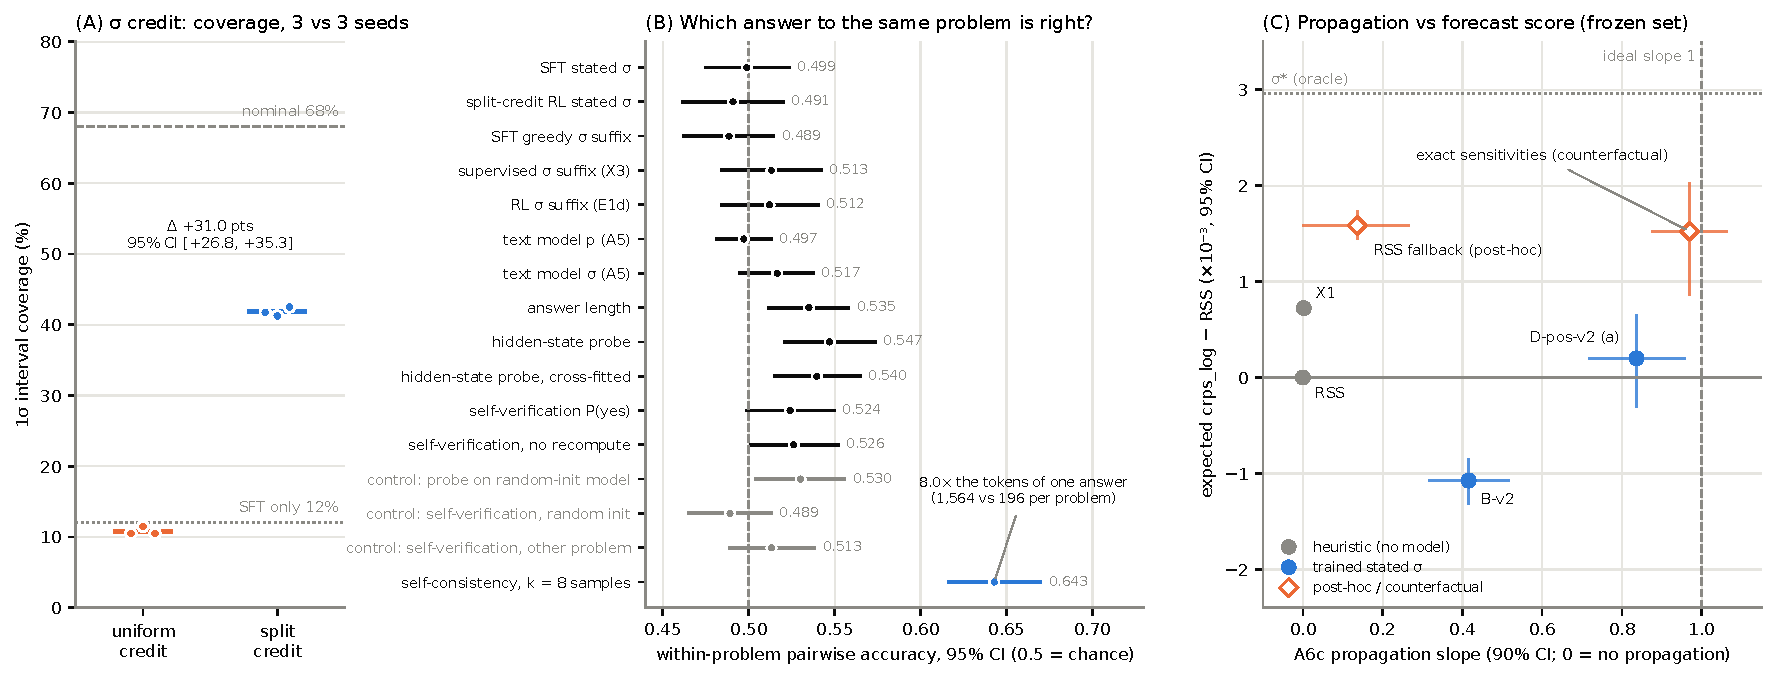
\includegraphics[width=\linewidth]{generated/figures/headline.pdf}
  % scripts/figures/headline.py via scripts/paper/figures.py; sources in paper/generated/SOURCES.md
  % (fig_headline); FINDINGS #18 (A), #19, #21, #22, #26, #37 (B), #32, #35, #36 (C).
  \caption{The three findings.
  (A) Uniform versus split credit: $1\sigma$ coverage per seed.
  (B) Within-problem pairwise accuracy of every correctness readout measured, against self-consistency.
  (C) On the frozen set, the noise-allocation slope against the expected-score difference from RSS.
  Every point is read from a committed result file; the sidecar \texttt{headline\_data.json} traces each one.}
  \label{fig:headline}
\end{figure}

\section{Does the model know which of its answers is right?}
\label{sec:act2}
\todo{To be written (docs/paper\_outline.md, section 5; FINDINGS \#7, \#19--\#22, \#26, \#37).}

% GENERATED by scripts/paper/tables.py; do not edit. Rebuild: uv run python scripts/paper/build.py
% artifact: table:cost
% sources (path @ git blob):
%   results/r5_diag/cost.json @ 364d31ae15dd
\begin{table}[t]
\centering
\small
\caption{Correctness signals against their inference cost.}
\label{tab:cost}
\begin{tabular}{@{}L{6.4cm} l r@{}}
\toprule
readout & pairwise accuracy [95\% CI] & tokens / problem \\
\midrule
self-consistency (agreement of the other samples) & \num{0.643} [\num{0.616}, \num{0.671}] & \num{1564} \\
hidden-state probe & \num{0.547} [\num{0.520}, \num{0.574}] & \num{196} \\
the same probe, random-init model & \num{0.530} [\num{0.503}, \num{0.557}] & \num{196} \\
completion length & \num{0.535} [\num{0.511}, \num{0.559}] & \num{196} \\
self-verification P(yes) (X4) & \num{0.524} [\num{0.498}, \num{0.550}] & \num{196} \\
stated $\sigma$ (SFT) & \num{0.499} [\num{0.474}, \num{0.524}] & \num{196} \\
\bottomrule
\end{tabular}
\par\smallskip\begin{minipage}{0.95\linewidth}\footnotesize Within-problem pairwise accuracy (a right answer ranked above a wrong one to the same problem; \num{516} problems, 95\% CIs clustered over problems) against generated tokens per problem (k = \num{8} samples for self-consistency). Source: results/r5\_diag/cost.json (FINDINGS \#22, \#37).\end{minipage}
\end{table}

% GENERATED by scripts/paper/tables.py; do not edit. Rebuild: uv run python scripts/paper/build.py
% artifact: table:cost_mca
% sources (path @ git blob):
%   results/r5_diag/cost.json @ 364d31ae15dd
\begin{table}[t]
\centering
\small
\caption{MC-A's spread against its cost, and MC-B's failure split.}
\label{tab:costmca}
\begin{tabular}{@{}l r r@{}}
\toprule
signal & AUROC & extra tokens / problem \\
\midrule
$\sigma^\star$ & \num{0.665} & \num{0} \\
RSS & \num{0.654} & \num{0} \\
X1 & \num{0.666} & \num{0} \\
B-v2 stated $\sigma$ & \num{0.655} & \num{0} \\
MC-A raw spread, $k=\num{2}$ & \num{0.638} & \num{496} \\
MC-A raw spread, $k=\num{4}$ & \num{0.710} & \num{992} \\
MC-A raw spread, $k=\num{8}$ & \num{0.745} & \num{1984} \\
\bottomrule
\end{tabular}
\par\smallskip\begin{minipage}{0.95\linewidth}\footnotesize A6c (development), AUROC of the signal for B-v2's run-0 answer being wrong, against the extra generated tokens per problem. MC-B's programs on the same set: \SI{79.7}{\percent} fail at the interface, \SI{5.1}{\percent} at run time, \SI{14.7}{\percent} run but compute the wrong chain, \SI{0.5}{\percent} are correct. Source: results/r5\_diag/cost.json (FINDINGS \#31, \#33, \#37).\end{minipage}
\end{table}


\section{Propagation of measurement noise: structure is not forecast quality}
\label{sec:act3}
\todo{To be written (docs/paper\_outline.md, section 6; FINDINGS \#17, \#23, \#27--\#39).}

% GENERATED by scripts/paper/tables.py; do not edit. Rebuild: uv run python scripts/paper/build.py
% artifact: table:confirmatory
% sources (path @ git blob):
%   results/stage_r4/confirmatory/results.json @ dc002a81d4ba
\begin{table}[t]
\centering
\small
\caption{The R4-3 confirmatory run: D-pos-v2 and B-v2 on the frozen set.}
\label{tab:confirmatory}
\begin{tabular}{@{}l L{5.2cm} l l l@{}}
\toprule
test & statistic & estimate [90\% CI] & $p$ & Holm \\
\midrule
K1 & D-pos-v2 (a): A6c slope $>0$ (primary) & \num{+0.816} [\num{+0.707}, \num{+0.923}] & \num{<1e-4} & rejected \\
K2 & D-pos-v2 (b) line's $X$: A6c slope $>0$ & \num{+0.884} [\num{+0.745}, \num{+1.041}] & \num{<1e-4} & rejected \\
K3 & D-pos-v2 (c) exact from terms: A6c slope $>0$ & \num{+0.843} [\num{+0.713}, \num{+0.987}] & \num{<1e-4} & rejected \\
K4 & B-v2: A6c slope $>0$ & \num{+0.416} [\num{+0.315}, \num{+0.517}] & \num{<1e-4} & rejected \\
K5 & D-pos-v2 $-$ B-v2 (expected crps\_log) & \num{+0.0013} [\num{+0.0008}, \num{+0.0017}] & \num{<1e-4} & rejected \\
K6 & D-pos-v2 $-$ RSS & \num{+0.0002} [\num{-0.0002}, \num{+0.0006}] & \num{0.201} & -- \\
K7 & D-pos-v2 $-$ X1 & \num{-0.0005} [\num{-0.0009}, \num{-0.0001}] & \num{0.991} & -- \\
K8 & B-v2 $-$ RSS & \num{-0.0011} [\num{-0.0013}, \num{-0.0009}] & \num{1.000} & -- \\
\midrule
C1--C3 & D-pos-v2 (a): A6b slope \num{+0.036} [\num{-0.057}, \num{+0.212}] & C1 yes, C2 yes, C3 yes & &  \\
C1--C3 & D-pos-v2 (b): A6b slope \num{-0.026} [\num{-0.049}, \num{-0.007}] & C1 yes, C2 yes, C3 yes & &  \\
C1--C3 & D-pos-v2 (c): A6b slope \num{-0.023} [\num{-0.047}, \num{-0.005}] & C1 yes, C2 yes, C3 yes & &  \\
C1--C3 & B-v2 (a): A6b slope \num{+0.003} [\num{-0.086}, \num{+0.129}] & C1 yes, C2 no, C3 yes & &  \\
\bottomrule
\end{tabular}
\par\smallskip\begin{minipage}{0.95\linewidth}\footnotesize Seed means over \num{3} seeds per arm, frozen R4-5 set (\num{3060} problems); stage B's joint pairs bootstrap, $B=\num{10000}$; 90\% CIs; one-sided $p$; Holm over K1--K8 at 0.05. Expected-score rows: oracle-centred expected crps\_log, pooled over the three sets, clustered over pairs. P = K1 $\wedge$ C2 $\wedge$ C3 (D125): confirmed. Source: results/stage\_r4/confirmatory/results.json (D118, D125; FINDINGS \#32).\end{minipage}
\end{table}

% GENERATED by scripts/paper/tables.py; do not edit. Rebuild: uv run python scripts/paper/build.py
% artifact: table:tail
% sources (path @ git blob):
%   results/r5_diag/tail.json @ d92087ff65fd
\begin{table}[t]
\centering
\small
\caption{Tail autopsy: what the worst problems get wrong.}
\label{tab:tail}
\begin{tabular}{@{}l r r@{}}
\toprule
primary cause & problem-seeds & share \\
\midrule
sensitivity: value-dependent: formula & \num{177} & \SI{39}{\percent} \\
sensitivity: value-dependent: substitution (own wrong intermediates) & \num{87} & \SI{19}{\percent} \\
copy: decimal shift & \num{71} & \SI{16}{\percent} \\
chain selection: wrong number of terms & \num{35} & \SI{8}{\percent} \\
sensitivity: power-law exponent & \num{28} & \SI{6}{\percent} \\
format: no answer $\sigma$ & \num{26} & \SI{6}{\percent} \\
sensitivity: value-dependent: formula (no expression) & \num{18} & \SI{4}{\percent} \\
format: no parsable $\sigma$ line & \num{7} & \SI{2}{\percent} \\
aggregation & \num{5} & \SI{1}{\percent} \\
sensitivity: transcription (S line right, $\sigma$-line coefficient wrong) & \num{1} & \SI{0}{\percent} \\
sensitivity: value-dependent: substitution (values) & \num{1} & \SI{0}{\percent} \\
\bottomrule
\end{tabular}
\par\smallskip\begin{minipage}{0.95\linewidth}\footnotesize D-pos-v2 (a), frozen R4-5 set, \num{3} seeds; the worst 5\% of problems by regret against $\sigma^\star$ per seed (\num{456} problem-seeds), classified by primary cause. They hold \SI{69}{\percent}--\SI{83}{\percent} of each seed's regret. Descriptive (R5-2, D133). Source: results/r5\_diag/tail.json (FINDINGS \#35).\end{minipage}
\end{table}

% GENERATED by scripts/paper/tables.py; do not edit. Rebuild: uv run python scripts/paper/build.py
% artifact: table:swaps
% sources (path @ git blob):
%   results/r5_diag/tail.json @ d92087ff65fd
\begin{table}[t]
\centering
\small
\caption{Component swaps: which part of the explicit $\sigma$ costs the score.}
\label{tab:swaps}
\begin{tabular}{@{}L{6.2cm} l r r@{}}
\toprule
$\sigma$ with & $-$ RSS [90\% CI] & gap closed & A6c slope \\
\midrule
(a) as stated & \num{+0.0002} [\num{-0.0002}, \num{+0.0006}] & \SI{7}{\percent} & \num{+0.837} \\
exact sensitivities (model's levels, aggregation, copy) & \num{+0.0015} [\num{+0.0010}, \num{+0.0020}] & \SI{51}{\percent} & \num{+0.970} \\
exact levels (model's sensitivities, aggregation, copy) & \num{+0.0002} [\num{-0.0002}, \num{+0.0006}] & \SI{7}{\percent} & \num{+0.838} \\
exact aggregation (model's terms and copy) & \num{-0.0008} [\num{-0.0016}, \num{-0.0001}] & \SI{-28}{\percent} & \num{+0.806} \\
exact copy, i.e. $\sigma$ = the line's X (= (b)) & \num{+0.0002} [\num{-0.0003}, \num{+0.0007}] & \SI{8}{\percent} & \num{+0.857} \\
model's terms, exact aggregation and copy (= (c)) & \num{-0.0018} [\num{-0.0040}, \num{-0.0002}] & \SI{-60}{\percent} & \num{+0.826} \\
fully exact: the builder's line, unrounded (ceiling) & \num{+0.0030} [\num{+0.0028}, \num{+0.0031}] & \SI{100}{\percent} & \num{+0.998} \\
\bottomrule
\end{tabular}
\par\smallskip\begin{minipage}{0.95\linewidth}\footnotesize One component of D-pos-v2's $\sigma$ replaced by its exact value at a time (R5-3, D133): a diagnostic of where the loss comes from, never a method. Slopes on every A6c pair, an unanswered member at the floor. RSS-to-$\sigma^\star$ gap \num{0.00296} (expected crps\_log). Source: results/r5\_diag/tail.json (FINDINGS \#35).\end{minipage}
\end{table}

% GENERATED by scripts/paper/tables.py; do not edit. Rebuild: uv run python scripts/paper/build.py
% artifact: table:llama
% sources (path @ git blob):
%   results/stage_xm/go_dpos2/go.json @ 2dda03c154a5
%   results/stage_xm/pilot/results.json @ ff891cafc25d
\begin{table}[t]
\centering
\small
\caption{The cross-model pilot on Llama-3.2-3B-Instruct.}
\label{tab:llama}
\begin{tabular}{@{}l L{5.6cm} L{5.0cm} l@{}}
\toprule
item & statistic & value & met \\
\midrule
K1, C2 & D-pos-v2 (a): A6c slope & \num{+0.785} [\num{+0.595}, \num{+0.974}] (\num{505} pairs) & yes, yes \\
C3 & D-pos-v2 (a): A6b slope, computation-correct pairs & \num{4} pairs: not measurable & no \\
go & K1 $\wedge$ C2 $\wedge$ C3 (D137) & & NO-GO \\
\midrule
desc. & A6b slope, all answered pairs (Llama / Qwen s0) & \num{-0.168} [\num{-0.220}, \num{-0.119}] / \num{+0.010} &  \\
desc. & B-v2 (a): A6c slope & \num{+0.396} [\num{+0.246}, \num{+0.544}] &  \\
desc. & D-pos-v2 $-$ B-v2 (expected crps\_log) & \num{-0.0089} [\num{-0.0170}, \num{-0.0019}] &  \\
format & D-pos-v2: parsed / units / computation-correct & \SI{99.8}{\percent} / \SI{99.7}{\percent} / \SI{8.0}{\percent} &  \\
format & B-v2: parsed / units / computation-correct & \SI{100.0}{\percent} / \SI{100.0}{\percent} / \SI{8.0}{\percent} &  \\
\bottomrule
\end{tabular}
\par\smallskip\begin{minipage}{0.95\linewidth}\footnotesize Seed 0, frozen A6c + A6b (D137, D146). The go rule is R4-3's criterion on D-pos-v2's answer $\sigma$; C3 needs at least three computation-correct A6b pairs. Descriptive rows are D137's, outside the go rule. Sources: results/stage\_xm/pilot/results.json, results/stage\_xm/go\_dpos2/go.json (FINDINGS \#38).\end{minipage}
\end{table}

% GENERATED by scripts/paper/tables.py; do not edit. Rebuild: uv run python scripts/paper/build.py
% artifact: table:j_results
% sources (path @ git blob):
%   results/r5_6/results.json @ 6195c81bfe0a
\begin{table}[t]
\centering
\small
\caption{R5-6 part J: Jacobians outside the training range of trained chains.}
\label{tab:j}
\begin{tabular}{@{}l L{4.3cm} L{5.6cm} l l@{}}
\toprule
test & statistic & estimate [90\% CI] & $p$ & Holm \\
\midrule
J1 & D-pos-v2 (a): J-sensitivity slope $>0$ (primary) & \num{+0.985} [\num{+0.868}, \num{+1.103}] & \num{<1e-4} & rejected \\
J2 & explicit $-$ implicit slope & \num{+0.530} [\num{+0.377}, \num{+0.676}] & \num{<1e-4} & rejected \\
J3 & D-pos-v2 $-$ RSS (expected crps\_log) & \num{+0.0011} [\num{-0.0002}, \num{+0.0020}] & \num{0.072} & -- \\
J4 & D-pos-v2 $-$ X1 & \num{+0.0000} [\num{-0.0013}, \num{+0.0008}] & \num{0.442} & -- \\
J5 & B-v2 $-$ RSS & \num{-0.0005} [\num{-0.0008}, \num{-0.0002}] & \num{0.997} & -- \\
J6 & B-v2 $-$ X1 & \num{-0.0016} [\num{-0.0019}, \num{-0.0013}] & \num{1.000} & -- \\
\midrule
source & D-pos-v2 (a) & sens.\ \num{+0.985} [\num{+0.868}, \num{+1.103}]; inv.\ \num{+0.026} [\num{-0.055}, \num{+0.119}] & \multicolumn{2}{l}{C1--C3: yes} \\
source & D-pos-v2 (b) & sens.\ \num{+1.007} [\num{+0.861}, \num{+1.172}]; inv.\ \num{+0.026} [\num{-0.028}, \num{+0.078}] & \multicolumn{2}{l}{C1--C3: yes} \\
source & D-pos-v2 (c) & sens.\ \num{+0.980} [\num{+0.835}, \num{+1.143}]; inv.\ \num{+0.004} [\num{-0.081}, \num{+0.082}] & \multicolumn{2}{l}{C1--C3: yes} \\
source & B-v2 (a) & sens.\ \num{+0.455} [\num{+0.348}, \num{+0.564}]; inv.\ \num{+0.184} [\num{-0.032}, \num{+0.400}] & \multicolumn{2}{l}{C1--C3: no} \\
comparator & $\sigma^\star$ & sens.\ \num{+1.000} [\num{+1.000}, \num{+1.000}] & &  \\
comparator & RSS & sens.\ \num{+0.000} [\num{+0.000}, \num{+0.000}] & &  \\
comparator & X1 & sens.\ \num{-0.001} [\num{-0.003}, \num{+0.002}] & &  \\
comparator & clamped to the training range & sens.\ \num{+0.831} [\num{+0.737}, \num{+0.919}] & &  \\
\bottomrule
\end{tabular}
\par\smallskip\begin{minipage}{0.95\linewidth}\footnotesize Seed means over \num{3} seeds per arm on the frozen J set (\num{1632} problems); bootstrap as Table~\ref{tab:confirmatory}; Holm over J1--J6. C3 uses computation-correct invariance pairs. P$_J$ = J1 $\wedge$ C2 $\wedge$ C3 (D147): confirmed. The clamped comparator propagates exactly but with every sensitivity clipped into its chain's training range. Source: results/r5\_6/results.json (D147; FINDINGS \#39).\end{minipage}
\end{table}

% GENERATED by scripts/paper/tables.py; do not edit. Rebuild: uv run python scripts/paper/build.py
% artifact: table:j_subgroups
% sources (path @ git blob):
%   results/r5_6/results.json @ 6195c81bfe0a
\begin{table}[t]
\centering
\footnotesize
\caption{R5-6 part J: J-sensitivity slopes where clamping matters most.}
\label{tab:jsub}
\begin{tabular}{@{}l r l l l@{}}
\toprule
subgroup & pairs & D-pos-v2 (a) & B-v2 (a) & clamped \\
\midrule
exceedance below the median & \num{408} & \num{+1.09} [\num{+0.96}, \num{+1.22}] & \num{+0.53} [\num{+0.37}, \num{+0.69}] & \num{+0.99} [\num{+0.91}, \num{+1.06}] \\
exceedance above the median & \num{408} & \num{+0.83} [\num{+0.63}, \num{+1.04}] & \num{+0.36} [\num{+0.22}, \num{+0.49}] & \num{+0.62} [\num{+0.45}, \num{+0.78}] \\
strict & \num{255} & \num{+0.89} [\num{+0.65}, \num{+1.12}] & \num{+0.39} [\num{+0.09}, \num{+0.72}] & \num{+0.71} [\num{+0.57}, \num{+0.85}] \\
rank flip & \num{43} & \num{+1.12} [\num{+0.88}, \num{+1.38}] & \num{+0.18} [\num{-0.13}, \num{+0.41}] & \num{+0.36} [\num{+0.00}, \num{+0.80}] \\
\bottomrule
\end{tabular}
\par\smallskip\begin{minipage}{0.95\linewidth}\footnotesize Descriptive, outside the Holm family (D147 \S10). Pairs: J-sensitivity and J-invariance pairs in the subgroup; slopes on the J-sensitivity pairs. Strict: also outside the range over every training chain to the same target. Rank flip: the dominant given was never dominant for that chain in training. Source: results/r5\_6/results.json.\end{minipage}
\end{table}


% Sections: Discussion and Limitations. NOT drafted yet (docs/paper_outline.md sections 7-8).
\section{Discussion}
\label{sec:discussion}
\todo{To be written (docs/paper\_outline.md, section 7).}

\section{Limitations}
\label{sec:limitations}
\todo{To be written (docs/paper\_outline.md, section 8): one model family; a synthetic domain; single-seed pilots;
fresh Jacobians only (D148); the Llama pilot's descriptive invariance slope.}


\bibliographystyle{plainnat}
\bibliography{refs}

\appendix
% Appendices. NOT drafted yet (docs/paper_outline.md appendices A and B).
\section{Pre-registration ledger}
\label{app:ledger}
\todo{Every pre-registered hypothesis marked supported, not supported, or not run (\path{docs/decision_timeline.md}).}

\section{Reproducibility}
\label{app:repro}
\todo{Reload and provenance checks, pinned bases, the bf16 merge pitfall, frozen-set checksums, compute
(docs/paper\_outline.md, appendix B). Every generated value, table and figure lists its committed sources in
\path{paper/generated/SOURCES.md}.}


\end{document}
